\begin{frame}{Бинарная запутанность}
  \begin{columns}
    \column{0.57\textwidth}
    \begin{block}{Критерии запутанности}
      \begin{itemize}
        \item Неравенства Белла \\
          {\footnotesize J.S. Bell \textit{Physics Physique Физика} \textbf{1}, 195 (1964)}
        \item Энтропия фон-Неймана \\
          {\footnotesize C.H.Bennett et al. \textit{Phys. Rev. A} \textbf{54}, 3824 (1996)}
        \item Критерий Вуттерса \\
          {\footnotesize W.K. Wootters, \textit{Phys. Rev. Lett.} \textbf{80}, 2245 (1998)}
        \item Мера Шмидта \\
          {\footnotesize Eisert J. and Briegel H. J. \textit{Phys. Rev. A} \textbf{64}, 022306 (2001)}
      \end{itemize}
    \end{block}
    
    \column{0.4\textwidth}
    \begin{figure}
      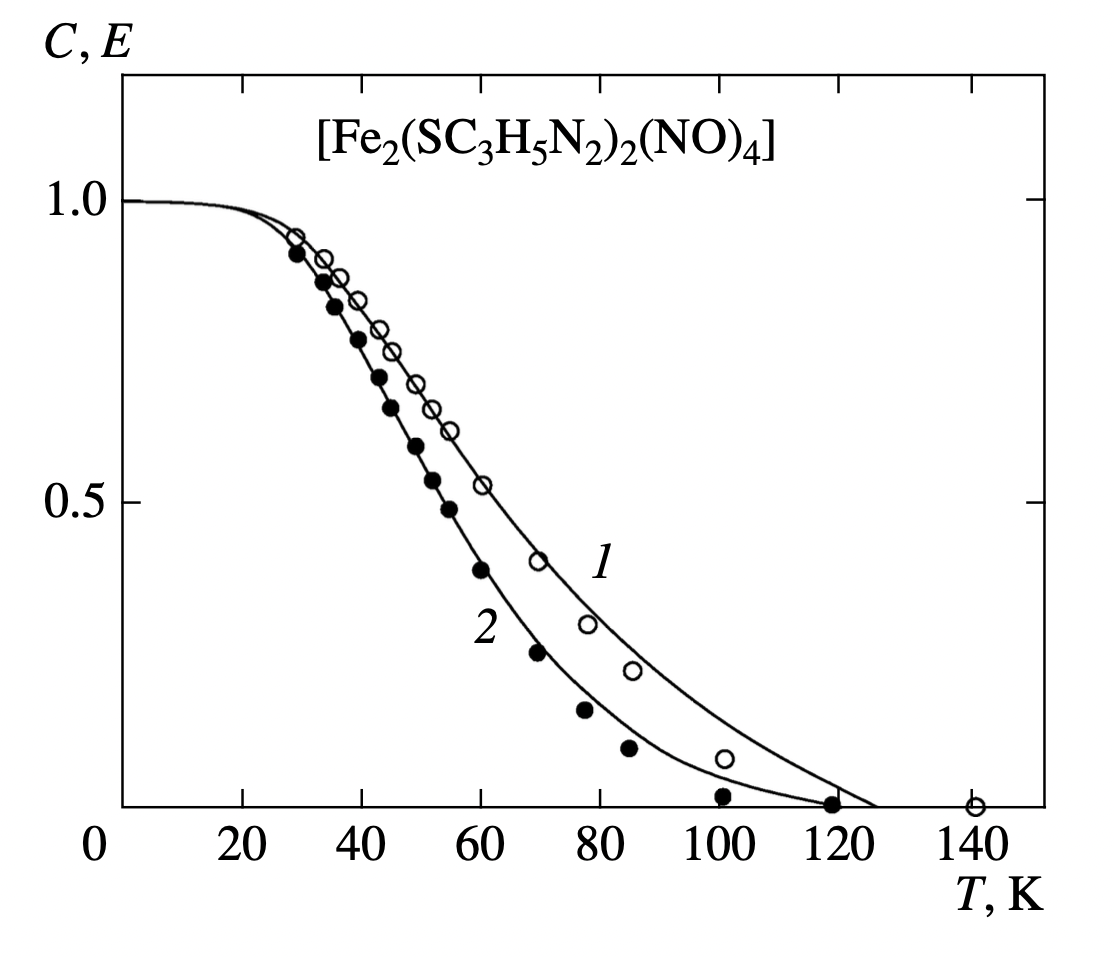
\includegraphics[width=\textwidth]{Aldoshin2008-concurence-by-temp.png}
      \captionsetup{skip=-2mm}
      \caption{Температурная зависимость согласованности (1) и запутанности (2) для нитрозильного комплекса железа\footnote[frame]{S. M. Aldoshin, E. B. Feldman, and M. A. Yurishchev, \textit{JETP} \textbf{107}, 5, 804–811 (2008)}.}
    \end{figure}
  \end{columns}
\end{frame}
\note{
  Классификация квантовых состояний на запутанные и сепарабельные нетривиальная задача.
  В действительности, чтобы показать, что состояние запутанно нужно еще угадать с проективными измерениями.
  В произвольном базисе можно упустить факт наличия запутанности.

  В случае состояния двух частиц задача классификации хорошо разработана
  и было предложено множество различных критериев и свидетелей.
  Самым первым критерием можно считать неравенства Белла. 
  
  Другие критерии, 
  в частности согласованность Вуттерса, 
  интересы потому что позволяют проследить связь запутанности с физическими наблюдаемыми параметрами.

  В качестве примера
  на слайде приведен результат из работы нашего института.
  Это температурная зависимость величины запутанности
  подсчитаной на основе согласованности Вуттерса в нитрозильном комплексе железа.
  Линии это теоретический расчет, точки это эксперимент.
  Такие результаты были получены благодаря тому, 
  что согласованность Вуттерса удалось связать с магнитной восприимчивостью атиферомагнитного димера.
}

\begin{frame}{Многочастичная запутанность}

Greenberger–Horne–Zeilinger
$$\ket{\mathrm{GHZ}} = \frac{\ket{000} + \ket{111}}{\sqrt{2}}$$

Wolfgang D\"ur
$$\ket{\mathrm{W}} = \frac{\ket{100} + \ket{010} +  \ket{001}}{\sqrt{3}}$$

$$
  \ket{\Psi}
  = \frac{1}{\sqrt{8}}
  \ket{0}
  \otimes
  \p{\ket{00} + \ket{11}}
  \otimes
  \p{\ket{000} + \ket{111}}
  \otimes
  \p{\ket{000} + \ket{111}}
$$
\end{frame}


% \begin{frame}{Квантовые технологии}
%   \begin{columns}
%    \column{0.6\textwidth}
%    \begin{figure}
%      \begin{subfigure}[t]{0.33\textwidth}
%        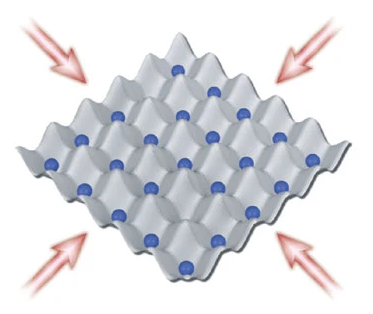
\includegraphics[width=\textwidth]{ultracold-atoms.png}
%        %\captionsetup{labelformat=empty}
%        \caption{Ultracold atoms}
%        \label{fig:ultracold-atoms}
%      \end{subfigure}
%      \begin{subfigure}[t]{0.33\textwidth}
%        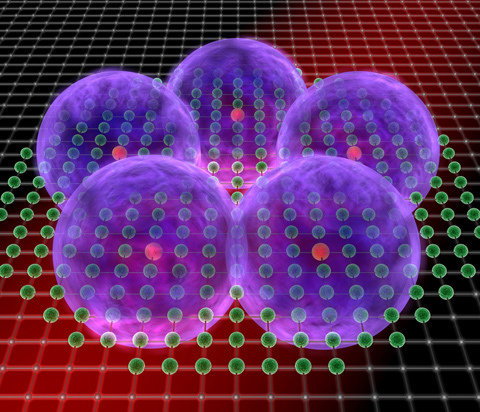
\includegraphics[width=\textwidth]{ridberg-atoms.png}
%        %\captionsetup{labelformat=empty}
%        \caption{Rydberg atoms}
%      \end{subfigure}
%      % \vspace*{2mm}
%      \vfill
%      \begin{subfigure}[t]{0.33\textwidth}
%        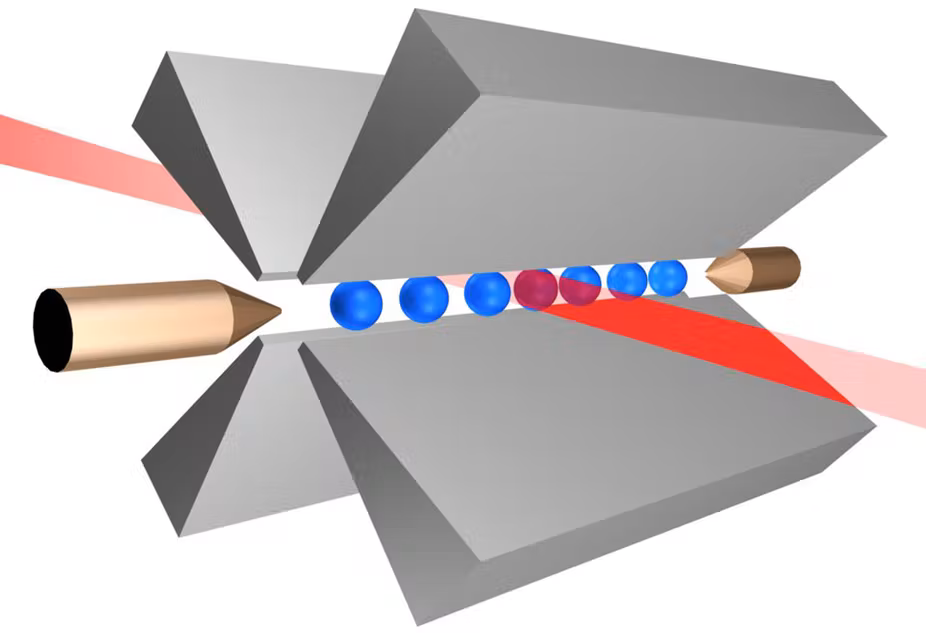
\includegraphics[width=\textwidth]{trapped-ions.png}
%        %\captionsetup{labelformat=empty}
%        \caption{Trapped ions}
%      \end{subfigure}
%      \begin{subfigure}[t]{0.33\textwidth}
%        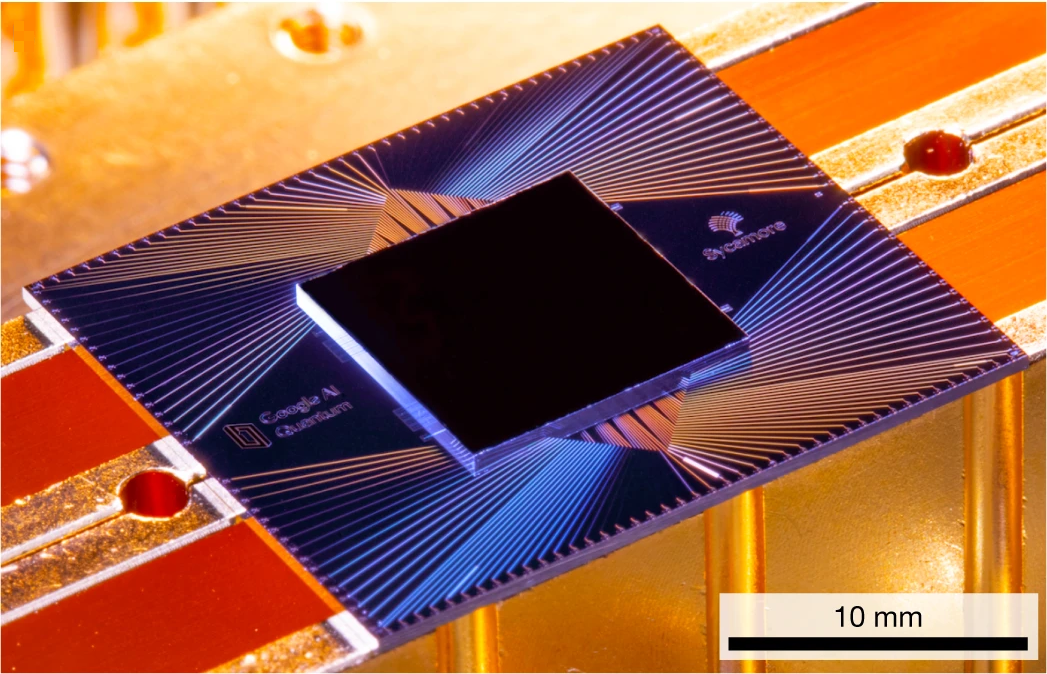
\includegraphics[width=\textwidth]{sycamore.png}
%        %\captionsetup{labelformat=empty}
%        \caption{SC qubits}
%      \end{subfigure}
%      \caption{
%        Квантовые платформы.
%        % (\ref{fig:ultracold-atoms})~{Bloch, I. Nature 453, 1016–1022 (2008)}
%      }
%    \end{figure}
% 
%    \column{0.4\textwidth}
%    \begin{figure}
%        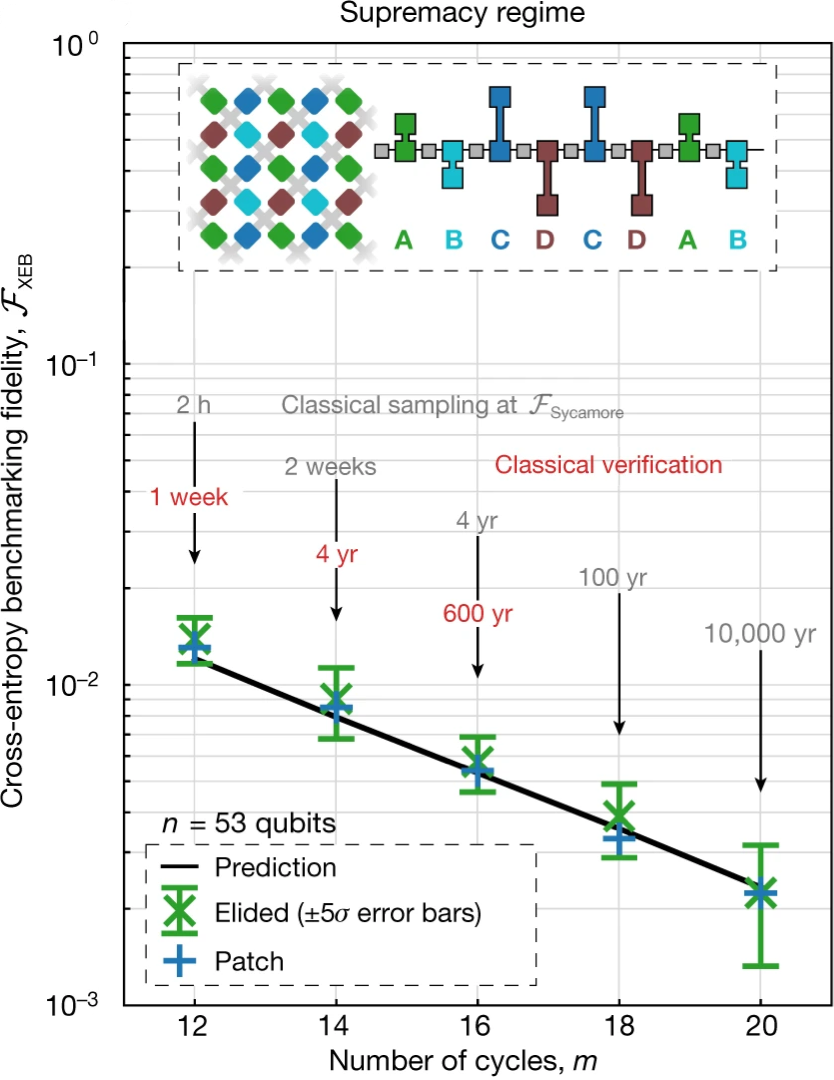
\includegraphics[width=0.8\textwidth]{sycamore-supemancy.png}
%        % \captionsetup{labelformat=empty}
%        \caption{
%          % F. Arute et al., Nature 574, 505 (2019)
%          Nature 574, 505 (2019)
%        }
%      \end{figure}
%    \end{columns}
% \end{frame}
% \note{
%   Тем неменее когда мы говорим о квантовом превосходстве
%   мы иммеем ввиду большое количество взаимодействующих кубитов.
%   Сейчас это порядка 50.
%   Это значит, что главным реусурсом является не бинарная запутанность, а многокубитная.
%   Предпринятые в данной работе попытки количественного определения запутанности мотивированы желанием понять и количественно оценить эти ресурсы.
% 
% 
%   % \textbf{ЯМР}
%   % ЯМР был первым, но он негодится для вычислений (нет чистых состояний).
%   % Отлично подходит для исследований.
%   % Много наработок.
% %
%   % Исследуется все гильбертого пространство.
%   % Квантовое превосходство  на программируемом сверхпроводящем процессоре.
%   % Запутанные состояния являются важным ресурсом в квантовых вычисления:
%   % Например, недавно продемонстрированное группой Мартинеса квантовое превосходство [1] на программируемом сверхпроводящем процессоре связано с понятием запутанноси
% }

